\documentclass{beamer}
\usepackage{cmbright,amssymb,amsmath,amsthm}
\usepackage{enumitem}
\usepackage{pinlabel}
\usepackage[tikz]{nmd/graphics}

\mode<presentation>{
\setbeamertemplate{frametitle}{
{\small\insertframetitle}\\
\vskip -14pt\hbox to \hsize{\hrulefill}
\par
}

\useinnertheme{circles}
\setbeamertemplate{navigation symbols}{}
}
\mode<all>

\newenvironment<>{thmblock}[1]{%
    \begin{actionenv}#2%
      \def\insertblocktitle{#1}%
      {\usebeamercolor[fg]{block title}\usebeamerfont{block title}\normalfont\insertblocktitle .}
   \end{actionenv}}

\def\inserttheoremblockenv{thmblock}
\parskip=10pt minus 6pt

\newtheorem{remark}[theorem]{Remark}
\newtheorem{proposition}[theorem]{Proposition}
\newtheorem{conjecture}[theorem]{Conjecture}
\newtheorem{question}[theorem]{Question}

\title{SnapPy - Part I}
\author{\vskip -40pt Marc Culler}
\newcommand\ZZ{{\mathbb Z}}
\newcommand\HH{{\mathbb H}}
\newcommand\QQ{{\mathbb Q}}
\newcommand\NN{{\mathbb N}}
\newcommand\RR{{\mathbb R}}
\newcommand\CC{{\mathbb C}}
\newcommand\PP{{\mathbb P}}
\newcommand\rank{\mathop{\rm rank}}
\newcommand\tr{\mathop{\rm tr}}
\newcommand\Hom{\mathop{\text{Hom}}}
\newcommand\vol{\text{vol}}
\newcommand\Vol{\text{Vol}}
\newcommand\fix{\text{fix}}
\newcommand\dist{\text{dist}}
\newcommand\inj{\text{inj}}
\newcommand\isom{{\text{Isom}_+}}
\newcommand\smear{\text{Smear}}
\newcommand\calI{\mathcal I}
\newcommand\calC{\mathcal C}
\newcommand\calH{\mathcal H}
\newcommand\calS{\mathcal S}
\newcommand\A{\mathcal A}
\newcommand\mer{\mathcal M}
\newcommand\lon{\mathcal L}
\newcommand\CS{\text{CS}_{\flat}}
\newcommand\SL{\text{SL}}
\newcommand\PSL{\text{PSL}}
\newcommand\SU{\text{SU}}
\newcommand\homeo{\text{Homeo}}
\newcommand\Hbar{\overline\HH}

\renewcommand{\today}{\vskip -48pt
Meudon, France\\30 May 2016}
\begin{document}

% Deal with pausing later
%\let\pause=\relax

\begin{frame}
\titlepage
\vskip -24pt
\pause
SnapPy is developed by  Marc Culler, Nathan Dunfield, Matthias Goerner,
and Jeff Weeks.  

With contributions from Mark Bell, Tracy Hall, Saul Schleimer, Malik
Obeidin, Robert Lipschitz, Jennet Dickinson and many others...
\end{frame}

\begin{frame}[t]
\frametitle{Hyperbolic $3$-Space}
Hyperbolic $3$-space $\HH^3$ is the unique homogeneous Riemannian
$3$-manifold with all sectional curvatures equal to
$-1$. Alternatively, $\HH^3 = PSL_2(\CC)/SO(3)$ with a normalized invariant metric.

There is a natural compactification
$\Hbar^3 \dot=\,\, \HH^3 \sqcup S^2_\infty$ which is homeomorphic
to a $3$-ball.  The boundary $S^2_\infty$ is the {\it sphere at
  infinity}.  It has a canonical conformal structure.

\pause
There are $8$ simply-connected Riemannian $3$-manifolds whose
full isometry group acts transitively with compact point stabilizers,
and which admit a compact quotient under the action of some discrete
torsion free group of isometries.  These are the ``geometries'' in
Thurston's Geometrization Conjecture, proved by Grisha Perelman in
2003.
\end{frame}

\begin{frame}[t]
\frametitle{Hyperbolic $3$-Space: {\it The Poincar\'e model}}
\begin{itemize}
\item[$\bullet$] $\HH^3$ is the open unit ball in $\RR^3$;
\pause
\item[$\bullet$] $S^2_\infty$ is the unit sphere;
\pause
\item[$\bullet$] A line is an arc of a circle which is perpendicular
  to $S^2_\infty$;
\pause
\item[$\bullet$] A plane is the intersection of the unit ball with a Euclidean
sphere perpendicular to $S^2_\infty$;
\pause
\item[$\bullet$] The metric is conformal to the Euclidean metric.
\end{itemize}
\end{frame}

\begin{frame}[t]
\frametitle{Hyperbolic $3$-Space: {\it The Poincar\'e model}}
{\large A convex polyhedron in the Poincar\'e model:}
\vskip 10pt
\centerline{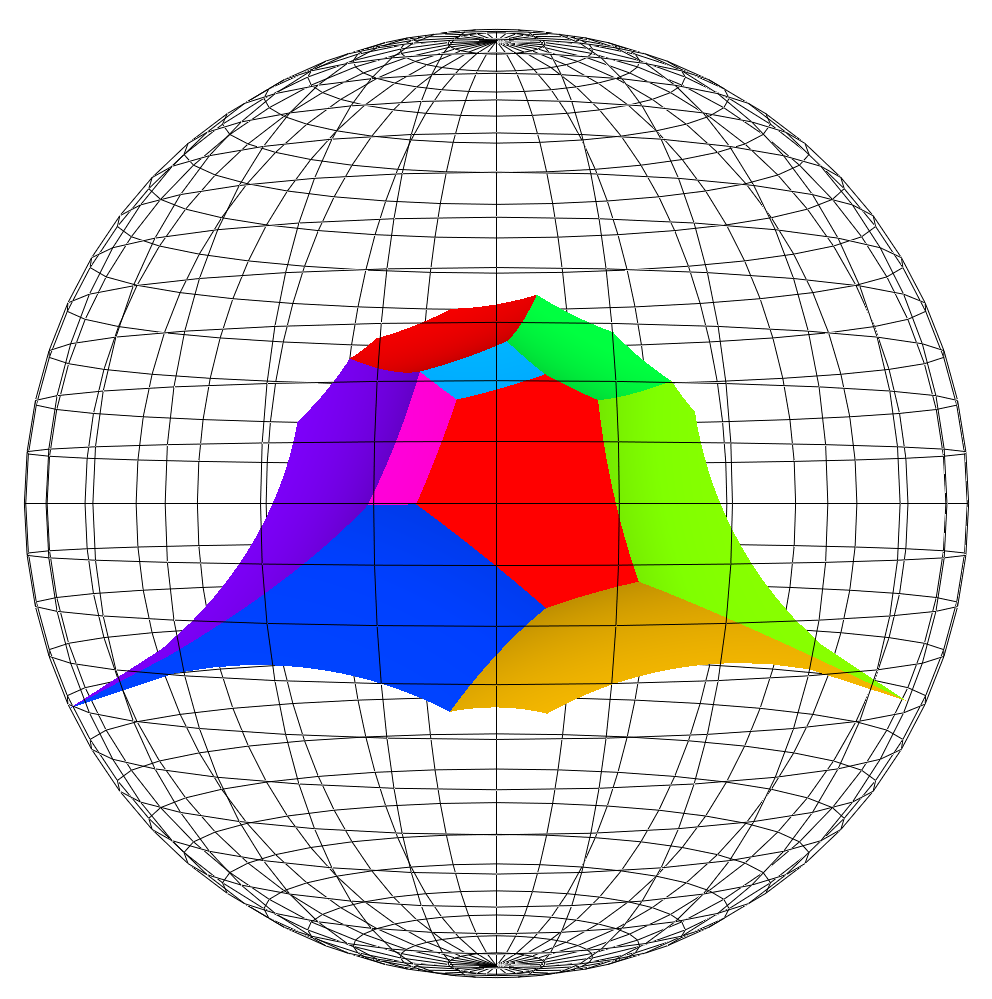
\includegraphics[height=.75\textheight]{Poincare.png}}
\end{frame}

\begin{frame}[t]
\frametitle{Hyperbolic $3$-Space: {\it The Klein model} }
\begin{itemize}
\item[$\bullet$] $\HH^3$ is the open unit ball in $\RR^3$;
\item[$\bullet$] $S^2_\infty$ is the unit sphere;
\item[$\bullet$] A line is the intersection of the ball with a Euclidean
line.
\item[$\bullet$] A plane is the intersection of the ball with a Euclidean
  plane.
\item[$\bullet$] The metric is {\it not} conformal to the Euclidean metric.
\end{itemize}
\end{frame}

\begin{frame}[t]
\frametitle{Hyperbolic $3$-Space: {\it The Klein model}}
{\large A convex polyhedron in the Klein model:}
\vskip 10pt
\centerline{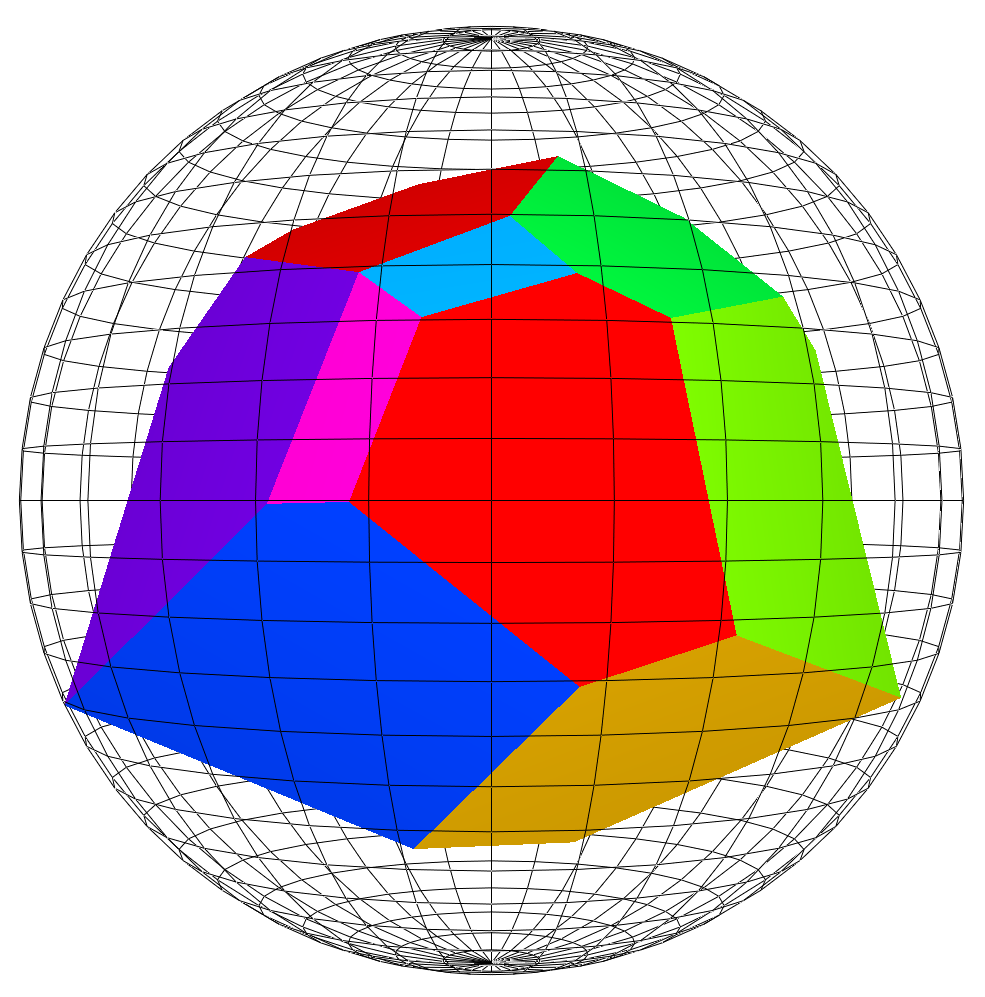
\includegraphics[height=.75\textheight]{Klein.png}}
\end{frame}

\begin{frame}[t]
\frametitle{Hyperbolic $3$-Space: {\it The upper half-space model:}}
\begin{itemize}
\item[$\bullet$] $\HH^3 = \{(x,y,t) | t > 0\} \subset \RR^3$;
\item[$\bullet$] $S^2_\infty$ is the plane $t=0$ together with the point $\infty$.
If the plane is identified with $\CC$, isometries of $\HH^3$ extend to M\"0bius
transformations on $\CC$ ($z \to \frac{az+b}{cz+d}$);
\item[$\bullet$] A line is a circle orthogonal to $t=0$, or a vertical line.
\item[$\bullet$] A plane is a half-sphere with center on $t=0$, or a vertical plane.
\item[$\bullet$] The metric is the Euclidean metric scaled by $\frac{1}{t}$.
\end{itemize}
\end{frame}

\begin{frame}[t]
\frametitle{Hyperbolic $3$-Space: {\it The upper half-space model}}
{\large An ideal tetrahedron in the upper half-space:}
\vskip 10pt
\centerline{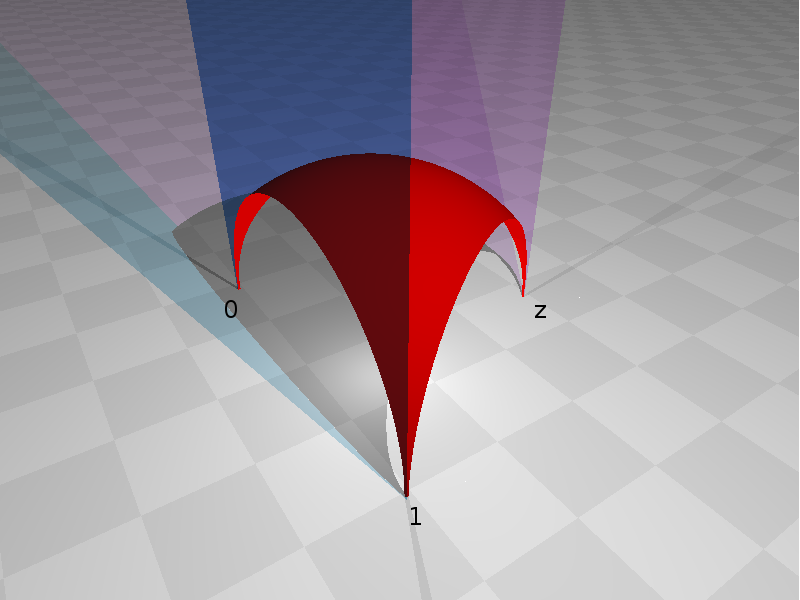
\includegraphics[height=.6\textheight]{labeledtet.png}}
This tetrahedron is the convex hull of the points $0$, $\infty$, $1$, $z$.
Up to isometry, every ideal tetrahedron has this form.
\end{frame}

\begin{frame}[t]
\frametitle{Hyperbolic $3$-Space: {\it Convex hulls}}
The closure in $\Hbar^3$ of a plane in $\HH^3$ is a $2$-disk whose
boundary is a geometric circle on $S^2_\infty$. Call this an extended plane.
\pause

Each extended plane in $\Hbar^3$ divides
$\Hbar$ into two closed half-spaces which meet along the extended
plane.  The {\it convex hull} of a subset $X$ of $\Hbar^3$ is the
intersection of all half-spaces containing $X$.  \pause

An {\it ideal tetrahedron} is the convex hull of four points on
$S^2_\infty$.  Every ideal tetrahedron has three symmetries which
interchange two pairs of opposite edges and reflect the other two
edges.
\pause

The cross-ratio of the vertices of an {\it ordered} ideal tetrahedron
is invariant under {\it order-preserving } isometries.  Take an ordered
tetrahedron $\Delta$ with cross-ratio $z$ and apply an order $2$ symmetry.
The new ordered tetrahedron will have cross-ratio $z$, $\frac{1}{1-z}$,
or $\frac{z-1}{z}$.
\pause

Remark: The boundary of the convex hull of any closed subset of
$S^2_\infty$ is a {\it pleated surface} bent along a {\it geodesic
  lamination}.
\end{frame}

\begin{frame}[t]
\frametitle{Hyperbolic $3$-Space: {\it Shapes}}

The {\it shape} of an ideal tetrahedron assigns complex numbers
to the edges in the following pattern.
\vskip -16pt
\begin{figure}[htb]
\labellist
\small\hair 2pt
 \pinlabel {$z$} at 22 87
 \pinlabel {$z$} at 127 41
 \pinlabel {$\frac{z-1}{z}$} at 41 10
 \pinlabel {$\frac{z-1}{z}$} at 104 115
 \pinlabel {$\frac1{1-z}$} at 80 90
 \pinlabel {$\frac1{1-z}$} at 108 65
 \pinlabel {$T_1$} at 275 78
 \pinlabel {$T_2$} at 248 93
 \pinlabel {$T_3$} at 223 80
 \pinlabel {$T_4$} at 222 50
 \pinlabel {$T_5$} at 248 36
 \pinlabel {$T_6$} at 273 50
\endlabellist
\centering
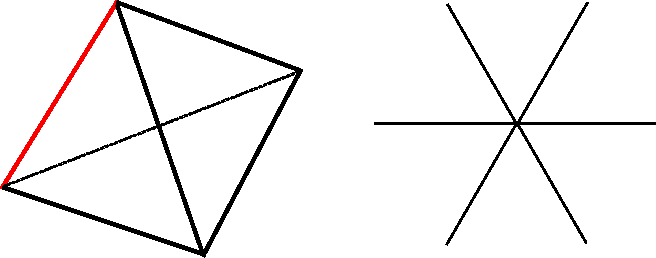
\includegraphics[width=\textwidth]{tetra}
\end{figure}
\pause
\vskip -16pt
If an ordered tetrahedron $\Delta = (v_0, v_1, v_2, v_3)$ is translated to
$(0, 1, \infty, z)$, then the shape assigns $z$ to the edge $v_0$ -- $v1$.
When $\operatorname{Im}(z)>0$ say that $\Delta$ is {\it positively oriented}. 
\pause

If tetrahedra $T_1, T_2, \ldots, T_n$ fit around an edge as shown, and
the shape values for that edge are $z_1, z_2, \ldots, z_n$, then
$z_1 \cdots z_n = 1$.
\medskip
\end{frame}

\begin{frame}[t]
\frametitle{Hyperbolic $3$-Space: {\it Volumes}}

Consider a co-compact discrete group $\Gamma$ of Euclidean translations of
$\RR^2$ with fundamental domain a parallelogram $P$.  The action extends
to an action by translations on $\RR^3$, which are isometries of the
upper half-space model.
\pause

The region $D$ = $P\times [1,\infty)$ is a fundamental domain for the action
of $\Gamma$ on $\RR^2\times [1,\infty)$.  The quotient is diffeomorphic to
$T^2\times[1,\infty)$ and inherits a complete hyperbolic metric.
The hyperbolic manifold, $D/\Gamma$ is called a {\it cusp neighborhood}.
A simple computation, using $dV_{\text{Hyp}} = \frac{1}{t^3}dV_{\text{Euc}}$, shows
that cusp neighborhoods have finite volume.
\pause

A $3$-manifold $M$ with a complete hyperbolic metric of finite volume
is either compact or has finitely many ends, each isometric to a
cusp neighborhood.  Thus $M$ is diffeomorphic to the interior of a
compact $3$-manifold with torus boundary components.
\end{frame}

\begin{frame}[t]
\frametitle{Hyperbolic $3$-Space: {\it Volumes}}
{\large A cusp neighborhood.}
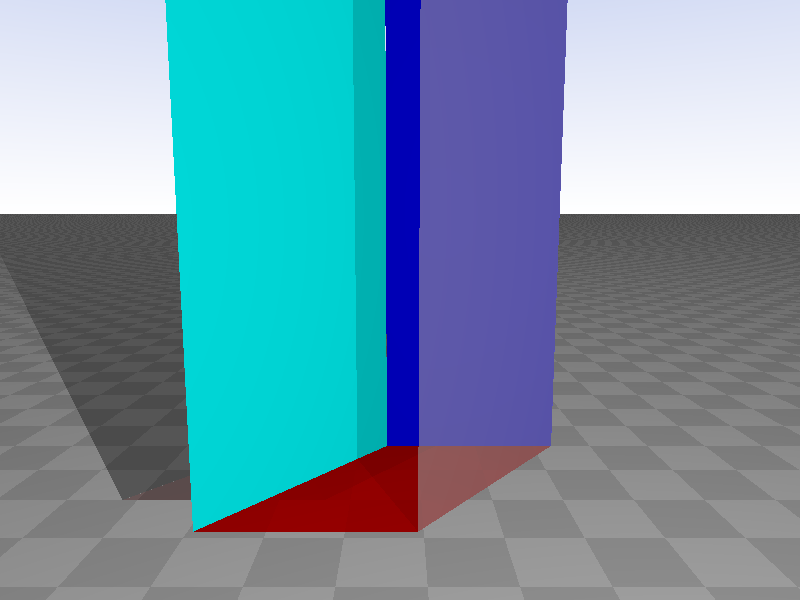
\includegraphics[height=0.75\textheight]{cusp.png}
\end{frame}

\begin{frame}[t]
\frametitle{Geometrization}
A $3$-manifold $M$ has a {\it geometric structure} if
\begin{itemize}
\item[$\bullet$] $M$ arises as the quotient of one of the $8$
  geometries by a discrete torsion-free group of isometries.
\item[$\bullet$] The induced Riemannian metric on $M$ is complete.
\end{itemize}
\pause
Every $3$-manifold is a connected sum of {\it irreducible} $3$-manifolds
which cannot be decomposed as a non-trivial connected sum.
 
\pause
The Geometrization Conjecture asserts that every compact irreducible
$3$-manifold with (possibly empty) torus boundary can be cut along
a canonical family of tori to produce (open) geometric manifolds.

\pause
For the $7$ non-hyperbolic geometries, the geometric manifolds
have been classified.

\pause
A finite volume hyperbolic $3$-manifold has a {\it unique} hyberbolic
structure by Mostow-Prasad rigidity.  So geometric invariants are
topological invariants. \pause (!!!!) 
\medskip
\end{frame}

\begin{frame}[t]
\frametitle{Computation}
SnapPy's data structure for representing a $3$-manifold $M$ contains:

An {\it ideal triangulation}:
\begin{itemize}
\item[$\bullet$] A pseudo-manifold $K$ constructed by identifying pairs of
  faces of finitely many tetrahedra so that every vertex link is either
  a sphere or a torus.  (To recover $M$, take the realization and
  delete the vertices with torus links.)
\item[$\bullet$] A complex shape parameter assigned to one edge of
  each tetrahedron. (The parameters for the other edges are determined.)
\end{itemize}
\pause
The shapes satisfy the {\it gluing equations}:
\begin{itemize}
\item[$\bullet$]For each equivalence class $e$ of edges, the product
  of the shapes assigned to the edges in $e$ equals $e^{2\pi i}$.
\end{itemize}
These equations have the simple form:
$$z_1^{a_1}(1-z_1)^{b_1} \cdots z_k^{a_k}(1-z_k)^{b_k} = c = \pm 1$$
\end{frame}

\begin{frame}[t]
\frametitle{Solving the gluing equations} 

The complex dimension of the space of solutions to the gluing
equations is equal to the number of cusps.  Adding a ``completeness
equation'' for each cusp cuts the dimension down to $0$, giving
finitely many solutions.
\pause

{\it In practice}, if the manifold has a hyperbolic structure then it
will be described by one of these finitely many solutions.  This means
that $M = \HH^3/\Gamma$ and there is a $\Gamma$-invariant tiling of
$\HH^3$ by tetrahedra of the specified shapes.
\pause

{\it In practice}, starting with all regular ideal tetrahedra,
Newton's method converges extremely quickly to the hyperbolic structure
(if one exists, as almost always happens).
\pause

Here is a plot of times required for computing hyperbolic structures
on knot complements, against the number of crossings in the knot diagram.
\end{frame}

\begin{frame}[t]
\frametitle{Time to compute volumes of knot complements}
  \matplotlibfigure[width=1.1\textwidth,
        font=\footnotesize]{volumetime}
\end{frame}

\begin{frame}[t]
\frametitle{Dehn filling} 
Without the completeness equations, solutions to the gluing equations
near the hyperbolic structure correspond to {\it incomplete} hyperbolic
structures.
\pause

Under certain conditions, the completion of one of these incomplete
metrics adds exactly a circle of points at the end of a cusp,
producing a hyperbolic manifold with different topology.
\pause

The topological operation, called {\it Dehn filling}, is: add a
boundary torus and then glue $S^1\times D^2$ to the new boundary
component.  The topology of the result is determined by the homotopy
class of the curve $\{*\}\times \partial D^2$ in the torus.  \pause

All but finitely many dehn fillings of a cusp yield a hyperbolic
manifold.  Finding the hyperbolic structure involves adding a {\it
  filling equation} instead of the completeness equation for the cusp.
Again, {\it in practice} Newton's method is amazingly effective.
\end{frame}

\begin{frame}[t]
\frametitle{Demo} 
\end{frame}

\begin{frame}[t]
\frametitle{Code profile}
  Under the hood, SnapPy is:
  \begin{itemize}
  \item C kernel: 40K LOC started by Weeks in 1990. 
  \item Cython wrapper: 5K LOC.
  \item Python code: 20K LOC.
  \item Databases with 2M+ manifolds.
  \item Modules hosted on PyPI.
  \item User-friendly native installers provided for OS X and Windows.    
  \end{itemize}
\emph{Why we're here: SnapPy and SageMath are friends!
  Nathan will expand on this after the break $\ldots$}
\end{frame}

\end{document}

